% Options for packages loaded elsewhere
\PassOptionsToPackage{unicode}{hyperref}
\PassOptionsToPackage{hyphens}{url}
%
\documentclass[
  ignorenonframetext,
]{beamer}
\usepackage{pgfpages}
\setbeamertemplate{caption}[numbered]
\setbeamertemplate{caption label separator}{: }
\setbeamercolor{caption name}{fg=normal text.fg}
\beamertemplatenavigationsymbolsempty
% Prevent slide breaks in the middle of a paragraph
\widowpenalties 1 10000
\raggedbottom
\setbeamertemplate{part page}{
  \centering
  \begin{beamercolorbox}[sep=16pt,center]{part title}
    \usebeamerfont{part title}\insertpart\par
  \end{beamercolorbox}
}
\setbeamertemplate{section page}{
  \centering
  \begin{beamercolorbox}[sep=12pt,center]{part title}
    \usebeamerfont{section title}\insertsection\par
  \end{beamercolorbox}
}
\setbeamertemplate{subsection page}{
  \centering
  \begin{beamercolorbox}[sep=8pt,center]{part title}
    \usebeamerfont{subsection title}\insertsubsection\par
  \end{beamercolorbox}
}
\AtBeginPart{
  \frame{\partpage}
}
\AtBeginSection{
  \ifbibliography
  \else
    \frame{\sectionpage}
  \fi
}
\AtBeginSubsection{
  \frame{\subsectionpage}
}
\usepackage{lmodern}
\usepackage{amssymb,amsmath}
\usepackage{ifxetex,ifluatex}
\ifnum 0\ifxetex 1\fi\ifluatex 1\fi=0 % if pdftex
  \usepackage[T1]{fontenc}
  \usepackage[utf8]{inputenc}
  \usepackage{textcomp} % provide euro and other symbols
\else % if luatex or xetex
  \usepackage{unicode-math}
  \defaultfontfeatures{Scale=MatchLowercase}
  \defaultfontfeatures[\rmfamily]{Ligatures=TeX,Scale=1}
\fi
% Use upquote if available, for straight quotes in verbatim environments
\IfFileExists{upquote.sty}{\usepackage{upquote}}{}
\IfFileExists{microtype.sty}{% use microtype if available
  \usepackage[]{microtype}
  \UseMicrotypeSet[protrusion]{basicmath} % disable protrusion for tt fonts
}{}
\makeatletter
\@ifundefined{KOMAClassName}{% if non-KOMA class
  \IfFileExists{parskip.sty}{%
    \usepackage{parskip}
  }{% else
    \setlength{\parindent}{0pt}
    \setlength{\parskip}{6pt plus 2pt minus 1pt}}
}{% if KOMA class
  \KOMAoptions{parskip=half}}
\makeatother
\usepackage{xcolor}
\IfFileExists{xurl.sty}{\usepackage{xurl}}{} % add URL line breaks if available
\IfFileExists{bookmark.sty}{\usepackage{bookmark}}{\usepackage{hyperref}}
\hypersetup{
  pdftitle={Lab Meeting},
  pdfauthor={Amy Van Scoyoc},
  hidelinks,
  pdfcreator={LaTeX via pandoc}}
\urlstyle{same} % disable monospaced font for URLs
\newif\ifbibliography
\usepackage{graphicx,grffile}
\makeatletter
\def\maxwidth{\ifdim\Gin@nat@width>\linewidth\linewidth\else\Gin@nat@width\fi}
\def\maxheight{\ifdim\Gin@nat@height>\textheight\textheight\else\Gin@nat@height\fi}
\makeatother
% Scale images if necessary, so that they will not overflow the page
% margins by default, and it is still possible to overwrite the defaults
% using explicit options in \includegraphics[width, height, ...]{}
\setkeys{Gin}{width=\maxwidth,height=\maxheight,keepaspectratio}
% Set default figure placement to htbp
\makeatletter
\def\fps@figure{htbp}
\makeatother
\setlength{\emergencystretch}{3em} % prevent overfull lines
\providecommand{\tightlist}{%
  \setlength{\itemsep}{0pt}\setlength{\parskip}{0pt}}
\setcounter{secnumdepth}{-\maxdimen} % remove section numbering

\title{Lab Meeting}
\subtitle{Coyote movement in human-modified landscapes}
\author{Amy Van Scoyoc}
\date{4/6/2022}

\begin{document}
\frame{\titlepage}

\begin{frame}{Dissertation Outline}
\protect\hypertarget{dissertation-outline}{}

\textbf{Theme:} \emph{Influence of human activity on landscapes and
predator-prey interactions}

\begin{itemize}
\tightlist
\item
  Ch. 1: Rapid islandization of Earth's protected areas (\emph{In Prep})
\item
  Ch. 2: Habitat edges drive animal movement in protected areas
  (\emph{TBD})
\item
  Ch. 3: The influence of human activity on predator-prey interactions
  (\emph{In Review})
\item
  Ch. 4: \textbf{Characterizing coyote resource selection in
  human-modified landscapes} (\emph{Analysis})
\end{itemize}


\includegraphics[width=0.25\textwidth,height=\textheight]{images/earth.png}
\includegraphics[width=0.25\textwidth,height=\textheight]{images/pathway.png}
\includegraphics[width=0.25\textwidth,height=\textheight]{images/human.png}
\includegraphics[width=0.25\textwidth,height=\textheight]{images/coyote.png}

\end{frame}

\begin{frame}{Research Objectives}
\protect\hypertarget{research-objectives}{}

Characterize the drivers of coyote behavior and resource selection at an
active sheep ranch.

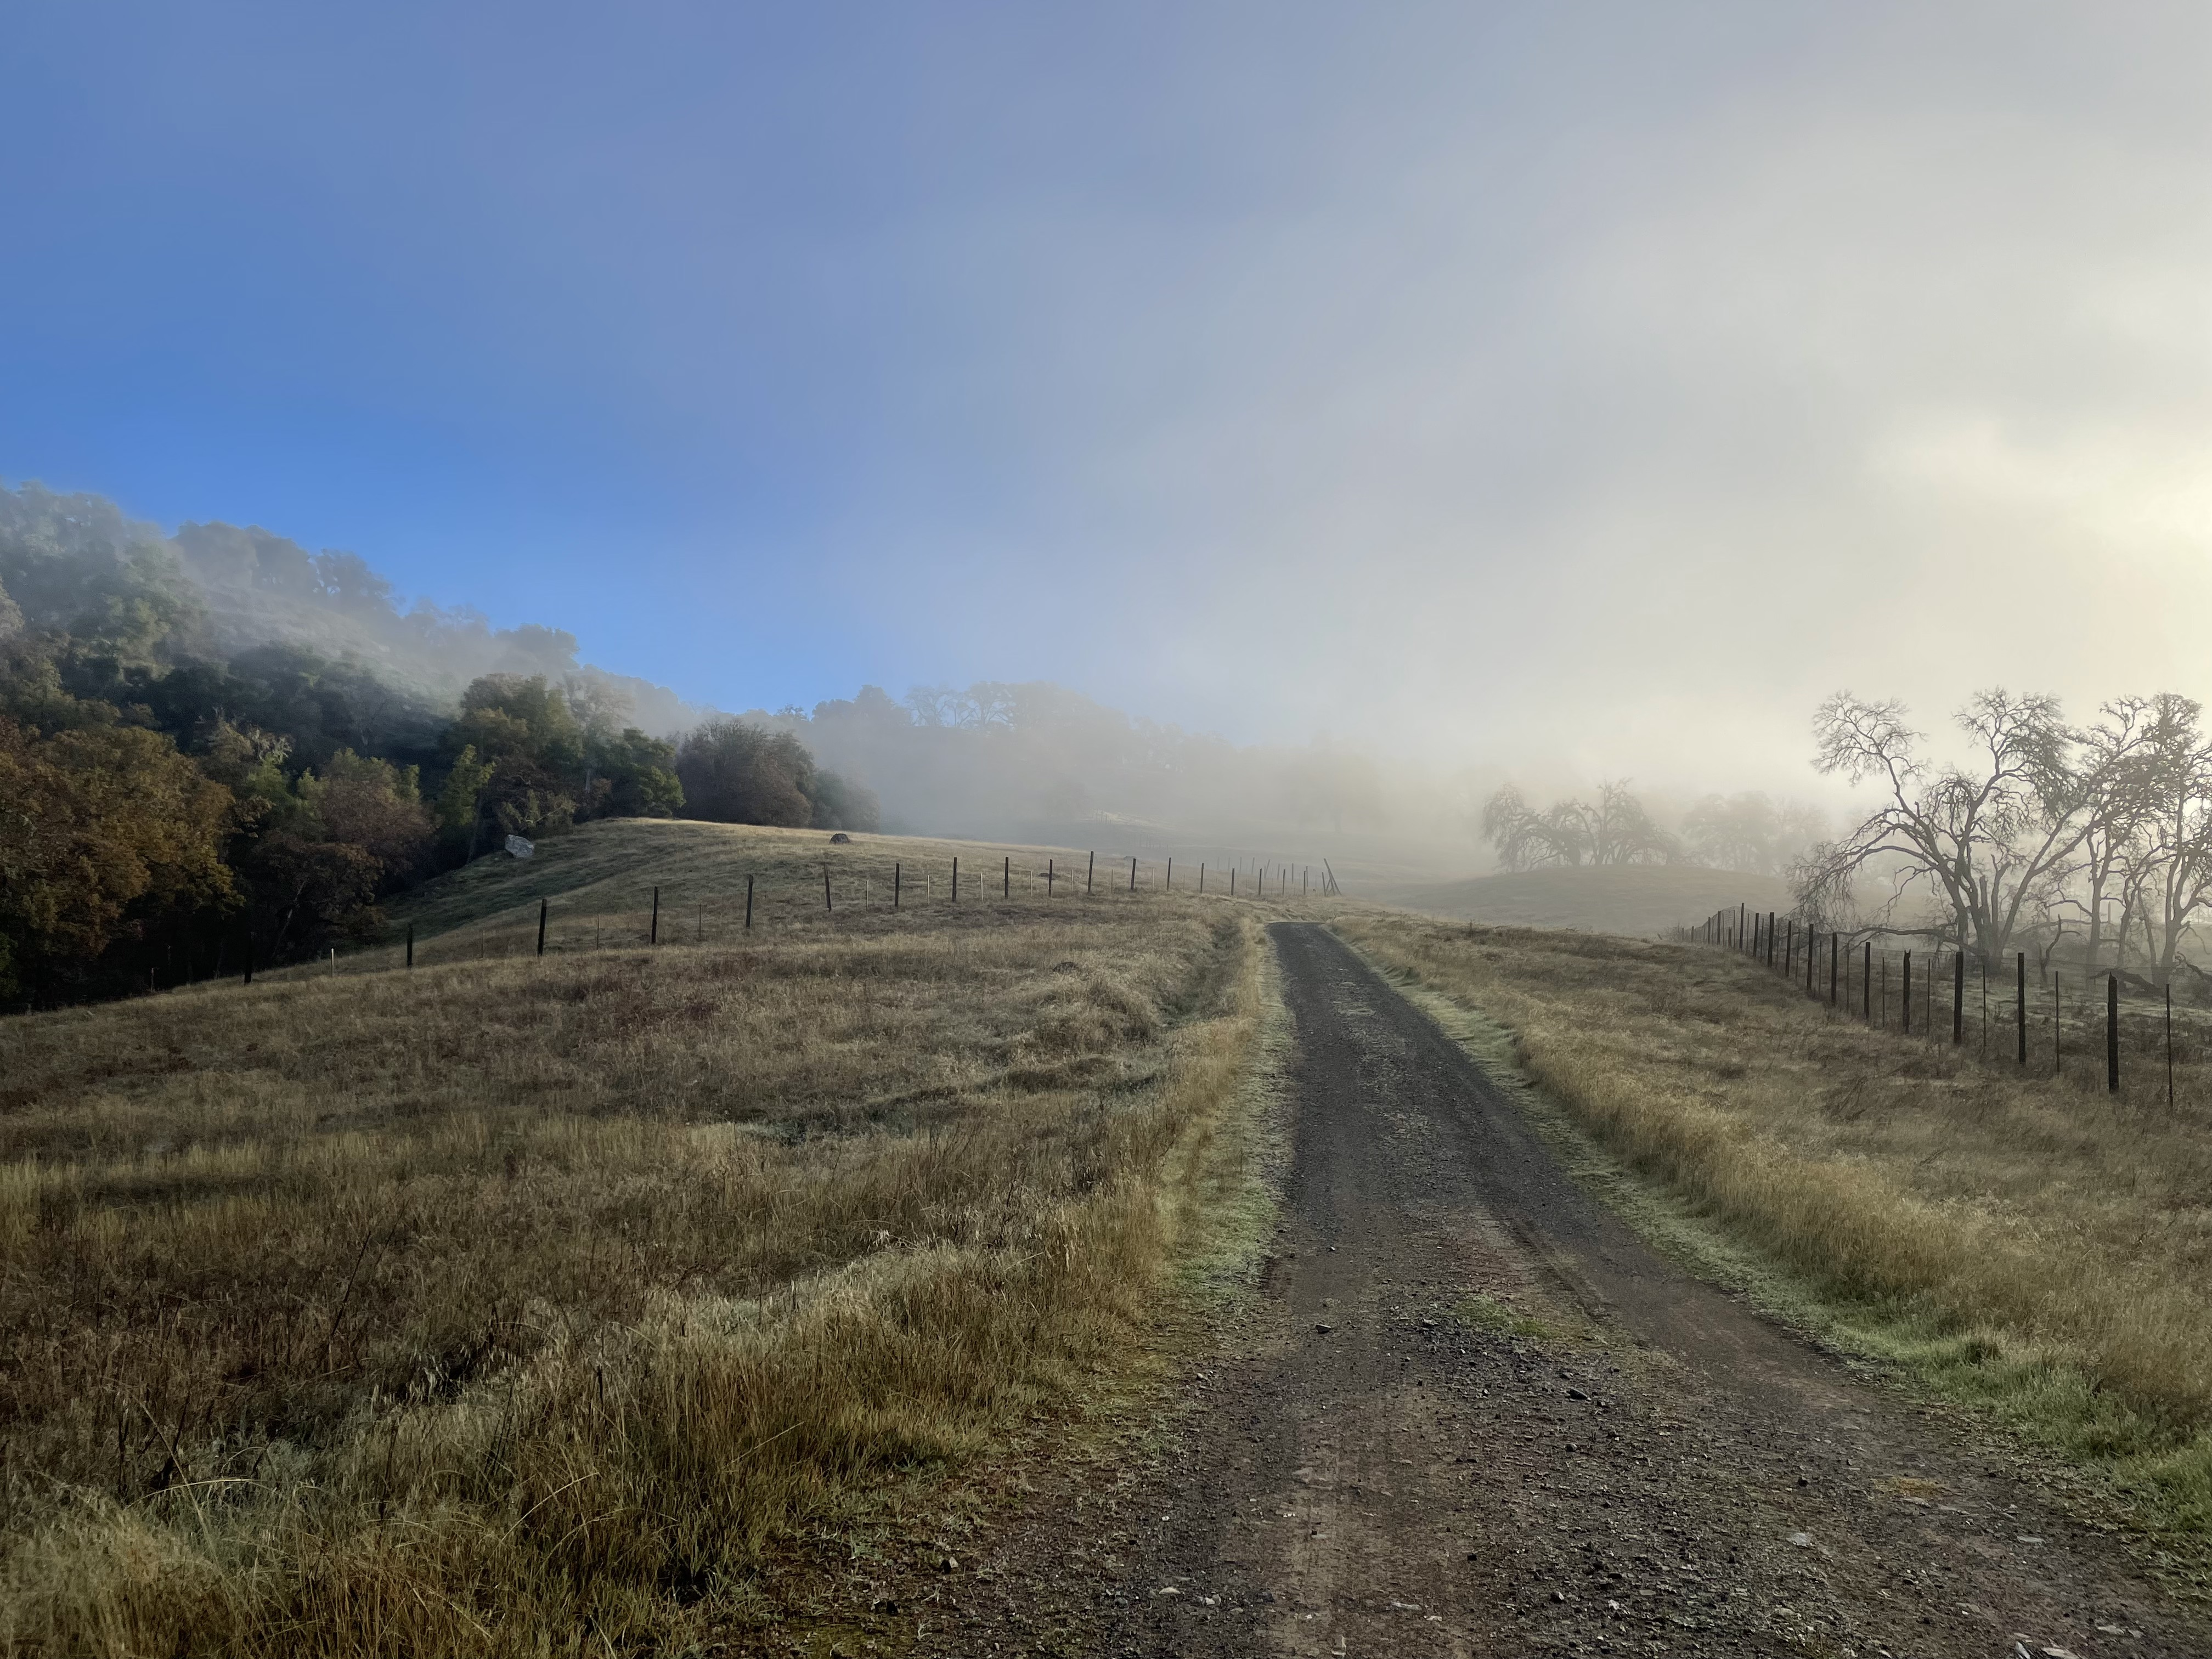
\includegraphics[width=0.6\textwidth,height=\textheight]{images/hopland.png}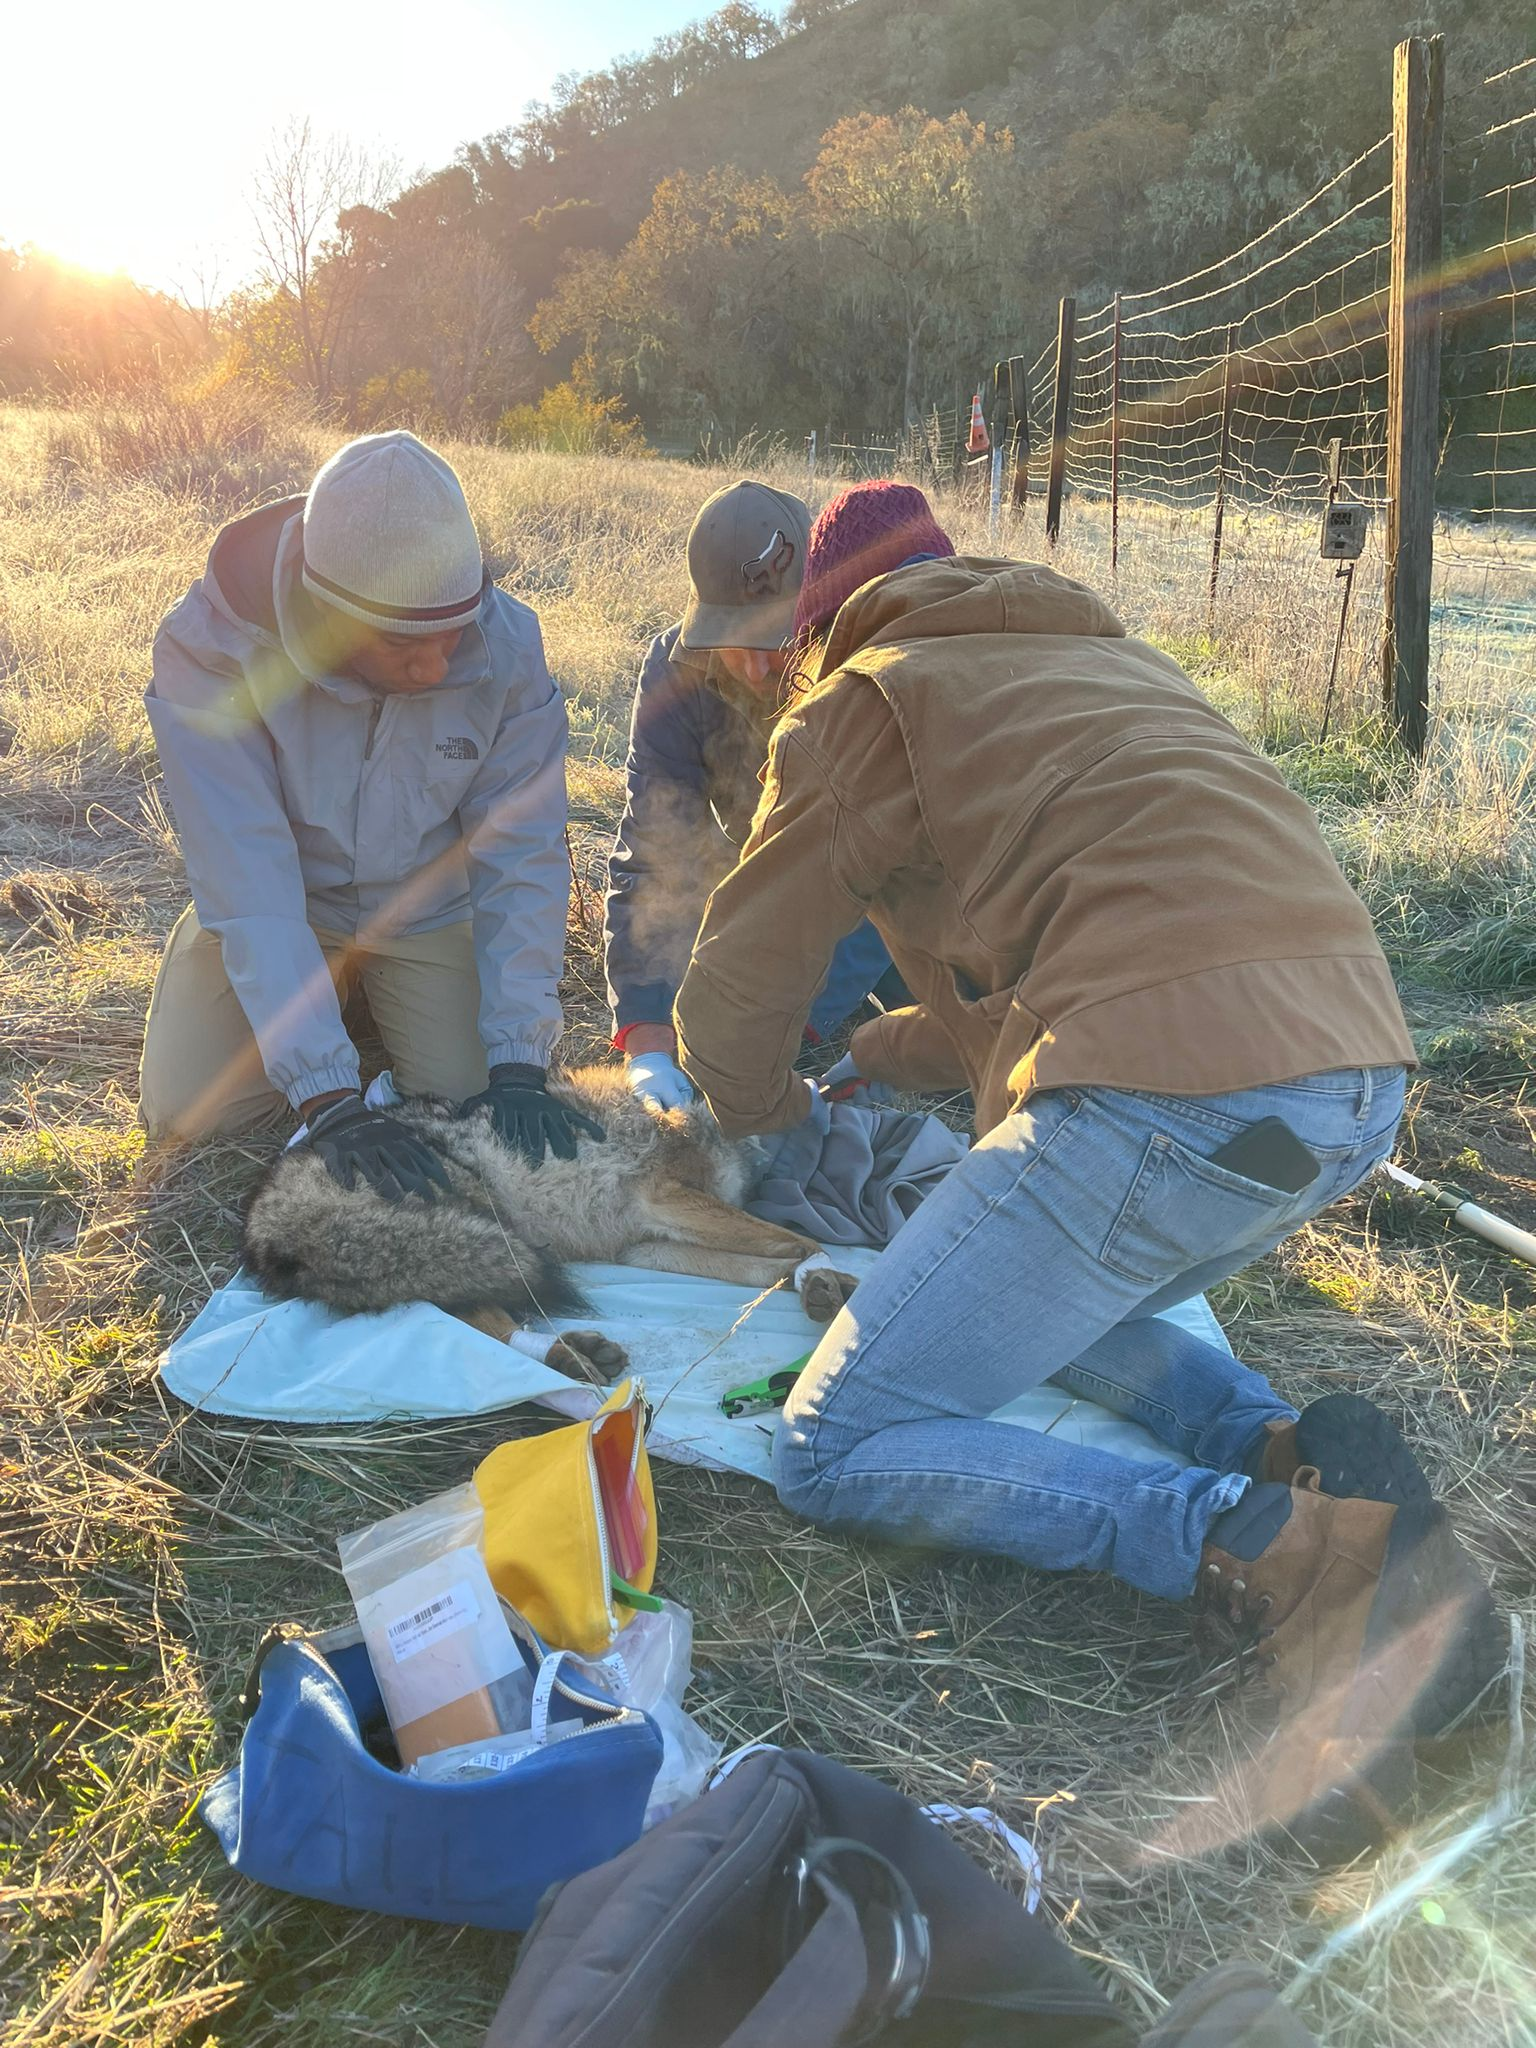
\includegraphics[width=0.34\textwidth,height=\textheight]{images/capture.png}

\end{frame}

\begin{frame}{Data Collection}
\protect\hypertarget{data-collection}{}

\textbf{Dataset:}

\begin{itemize}
\tightlist
\item
  2 field seasons, December - March
\item
  8 coyotes, 1-hour fix rate
\item
  4 guardian dogs, 10-min fix rate
\end{itemize}

\textbf{Notes:}

\begin{itemize}
\tightlist
\item
  Lambs in pasture February - March
\item
  Grapes in season August - November
\end{itemize}

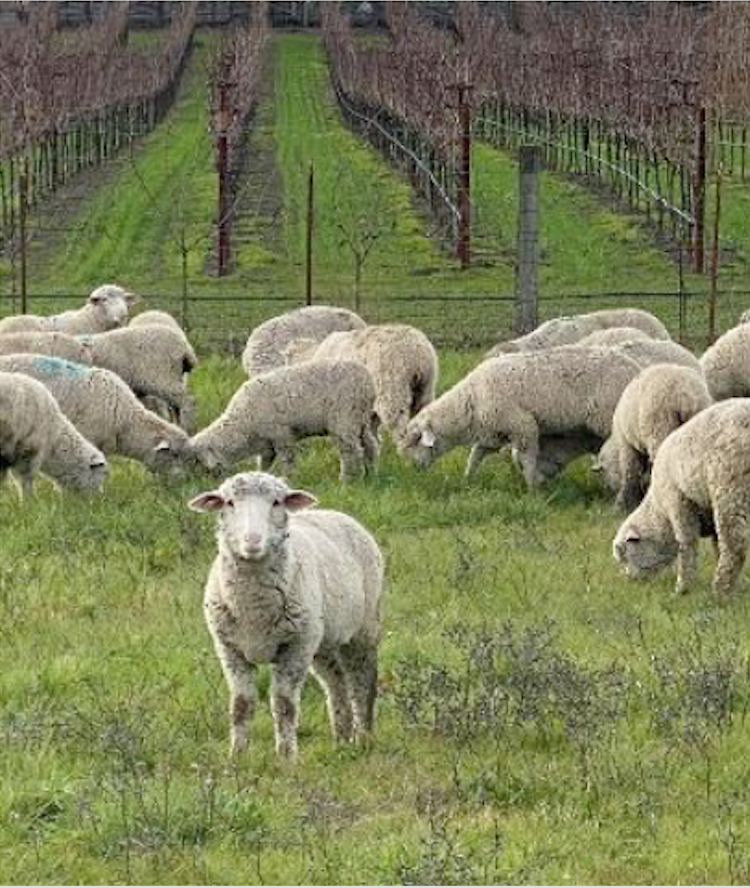
\includegraphics[width=0.8\textwidth,height=\textheight]{images/grape.png}

\end{frame}

\begin{frame}{Coyote Home Ranges}
\protect\hypertarget{coyote-home-ranges}{}

These are the 95\% Kernel Utilization Distributions for 2 seasons of
coyotes (n = 9).

\includegraphics{Presentation_files/figure-beamer/unnamed-chunk-2-1.pdf}

\end{frame}

\begin{frame}{Covariates}
\protect\hypertarget{covariates}{}

There are several environmental variables that may influence coyote
resource selection, including:

\begin{tabu} to \linewidth {>{\raggedright}X>{\raggedright}X}
\hline
\begingroup\fontsize{30}{32}\selectfont Physical\endgroup & \begingroup\fontsize{30}{32}\selectfont Other\endgroup\\
\hline
Land use & Day/Night\\
\hline
Slope & Lamb presence\\
\hline
Elevation & Guard Dog home range\\
\hline
Distance to water & Grape presence\\
\hline
\end{tabu}

\end{frame}

\begin{frame}{Covariates}
\protect\hypertarget{covariates-1}{}

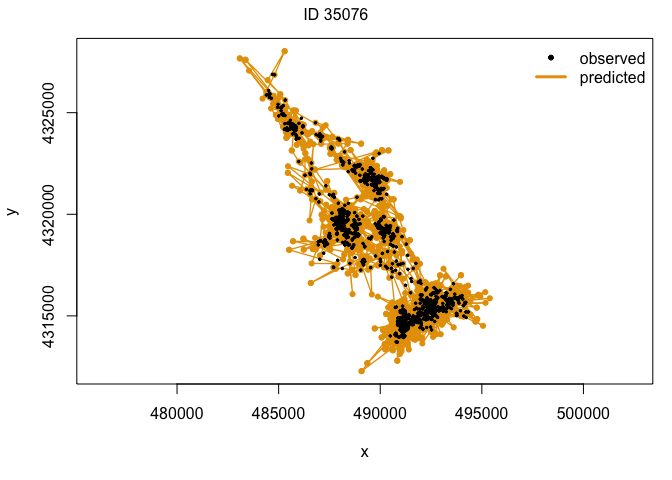
\includegraphics{Presentation_files/figure-beamer/unnamed-chunk-5-1.pdf}

\end{frame}

\begin{frame}{Step Selection Functions (SSF)}
\protect\hypertarget{step-selection-functions-ssf}{}

A first pass: \textbf{Land Use}

\emph{How do coyotes use cropland and natural areas?}

Steps inspired by Abrahms et al.~2016:

\begin{enumerate}
\tightlist
\item
  Use HMM to parse into three behavioral states (resting, traveling,
  meandering).
\item
  Create a SSF for all movement data without parsing by behavior
  (`combined model')
\item
  Create SSFs for movement by behavior (`behavior model')
\item
  Compare
\end{enumerate}

\end{frame}

\begin{frame}{Hidden Markov Models (HMM)}
\protect\hypertarget{hidden-markov-models-hmm}{}

Hidden markov models can use distance traveled and angles between time
points to infer behavioral states of animals.

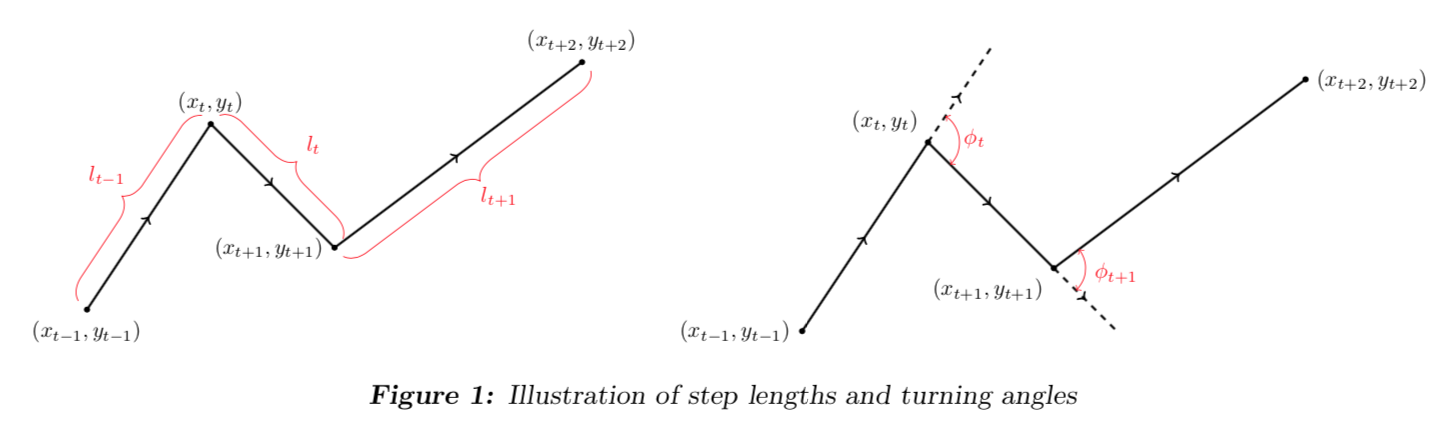
\includegraphics[width=0.75\textwidth,height=\textheight]{images/steps_angles.png}

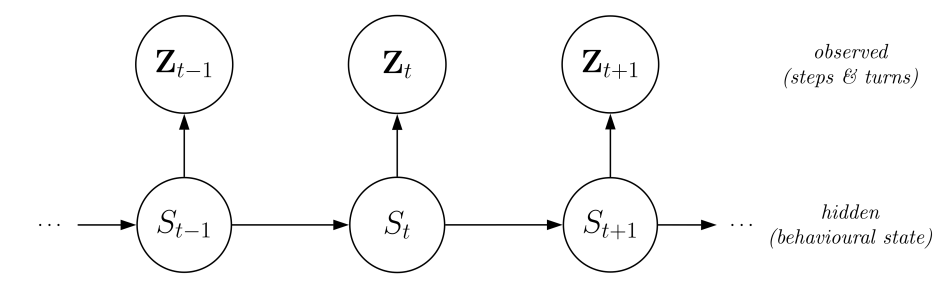
\includegraphics[width=0.75\textwidth,height=\textheight]{images/hmm.png}

\end{frame}

\begin{frame}{Hidden Markov Models (HMM)}
\protect\hypertarget{hidden-markov-models-hmm-1}{}

Initial parameters ranges for 3 states:

\begin{tabu} to \linewidth {>{\raggedright}X>{\raggedleft}X>{\raggedleft}X>{\raggedleft}X>{\raggedleft}X>{\raggedleft}X>{\raggedleft}X>{\raggedleft}X}
\hline
\begingroup\fontsize{20}{22}\selectfont State\endgroup & \begingroup\fontsize{20}{22}\selectfont SL\_min\endgroup & \begingroup\fontsize{20}{22}\selectfont SL\_max\endgroup & \begingroup\fontsize{20}{22}\selectfont SD\_min\endgroup & \begingroup\fontsize{20}{22}\selectfont SD\_max\endgroup & \begingroup\fontsize{20}{22}\selectfont TA\endgroup & \begingroup\fontsize{20}{22}\selectfont Conc\_min\endgroup & \begingroup\fontsize{20}{22}\selectfont Conc\_max\endgroup\\
\hline
Resting & 50 & 100 & 25 & 50 & 3.141593 & 0.2 & 0.5\\
\hline
Meandering & 500 & 1000 & 250 & 500 & 1.570796 & 0.5 & 0.7\\
\hline
Traveling & 1000 & 3000 & 500 & 1500 & 0.000000 & 0.7 & 3.0\\
\hline
\end{tabu}

\end{frame}

\begin{frame}[fragile]{Hidden Markov Models (HMM)}
\protect\hypertarget{hidden-markov-models-hmm-2}{}

Here are the parameters for the best HMM (n = 25 iterations), with the
lowest AIC.

\begin{verbatim}
## [1] "Step Parameters:"
\end{verbatim}

\begin{verbatim}
##                state 1      state 2      state 3
## mean      2.582279e+01 1.869097e+02 7.724008e+02
## sd        1.963225e+01 1.589263e+02 5.841408e+02
## zero-mass 4.166166e-04 1.010215e-03 2.473974e-04
\end{verbatim}

\begin{verbatim}
## [1] "Angle Parameters:"
\end{verbatim}

\begin{verbatim}
##                 state 1   state 2     state 3
## mean          3.0936337 3.0003092 -0.05766519
## concentration 0.4500531 0.3069862  0.33858379
\end{verbatim}

\end{frame}

\begin{frame}[fragile]{Hidden Markov Models (HMM)}
\protect\hypertarget{hidden-markov-models-hmm-3}{}

\begin{verbatim}
## Decoding states sequence... DONE
\end{verbatim}

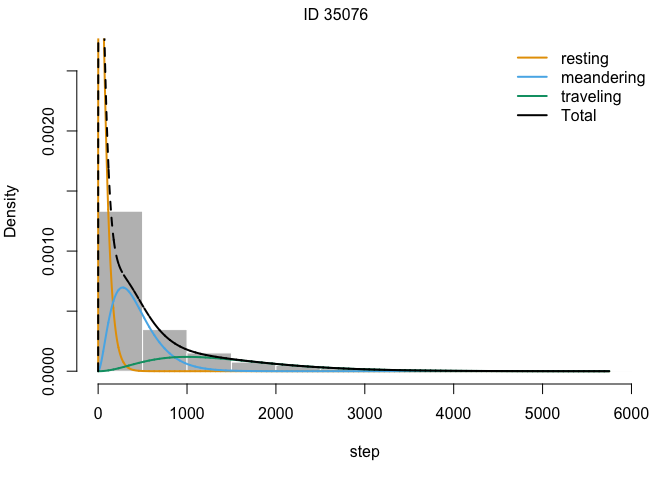
\includegraphics{Presentation_files/figure-beamer/unnamed-chunk-8-1.pdf}
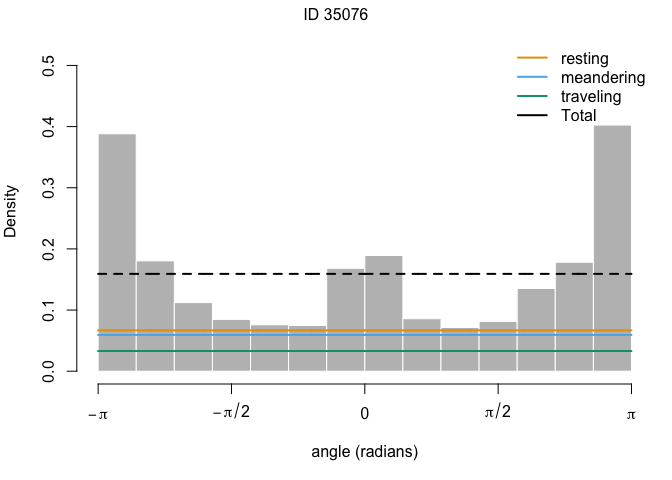
\includegraphics{Presentation_files/figure-beamer/unnamed-chunk-8-2.pdf}
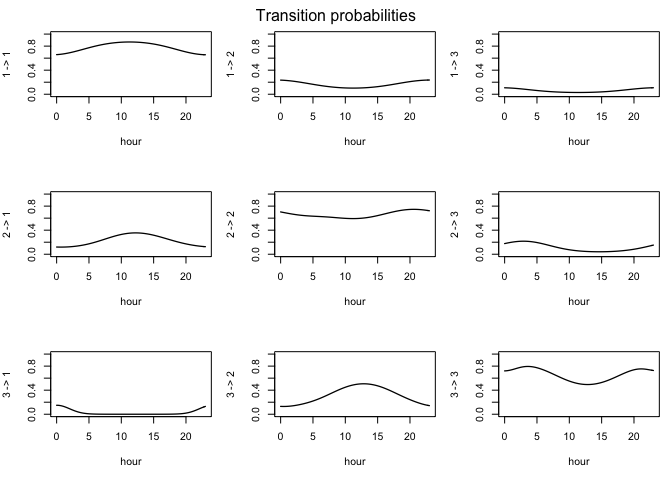
\includegraphics{Presentation_files/figure-beamer/unnamed-chunk-8-3.pdf}
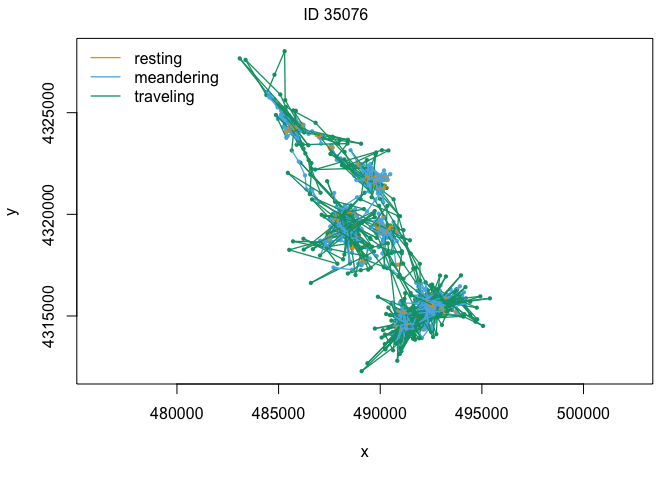
\includegraphics{Presentation_files/figure-beamer/unnamed-chunk-8-4.pdf}
\includegraphics{Presentation_files/figure-beamer/unnamed-chunk-8-5.pdf}
\includegraphics{Presentation_files/figure-beamer/unnamed-chunk-8-6.pdf}
\includegraphics{Presentation_files/figure-beamer/unnamed-chunk-8-7.pdf}
\includegraphics{Presentation_files/figure-beamer/unnamed-chunk-8-8.pdf}
\includegraphics{Presentation_files/figure-beamer/unnamed-chunk-8-9.pdf}
\includegraphics{Presentation_files/figure-beamer/unnamed-chunk-8-10.pdf}
\includegraphics{Presentation_files/figure-beamer/unnamed-chunk-8-11.pdf}

\end{frame}

\begin{frame}[fragile]{Hidden Markov Models (HMM)}
\protect\hypertarget{hidden-markov-models-hmm-4}{}

We can append the inferred state to the dataframe:

\begin{verbatim}
## # A tibble: 6 x 7
##   ID     step  angle       x        y time                states
##   <chr> <dbl>  <dbl>   <dbl>    <dbl> <dttm>               <dbl>
## 1 C4    358.  NA     494641. 4319299. 2021-02-28 17:00:15      2
## 2 C4    388.   0.289 494510. 4318966. 2021-02-28 16:00:16      2
## 3 C4    332.  -1.63  494477. 4318580. 2021-02-28 15:00:12      2
## 4 C4    141.   2.36  494148. 4318628. 2021-02-28 14:00:30      2
## 5 C4     34.2 -1.51  494233. 4318514. 2021-02-28 13:00:19      1
## 6 C4     20.9 -0.601 494207. 4318492. 2021-02-28 12:00:19      1
\end{verbatim}

\end{frame}

\begin{frame}{Step Selection Functions (SSF)}
\protect\hypertarget{step-selection-functions-ssf-1}{}

\textbf{Model structure:} \emph{amt::fit\_issf(steps, case\_
\textasciitilde{} landuse\_end + strata(step\_id\_))}

Table 1.Summary of step selection coefficients for `Land Use' by
behavior category (n = 7 individuals)

\begin{table}
\centering
\begin{tabular}{l|l|r|r|r|r}
\hline
\begingroup\fontsize{20}{22}\selectfont Behavioral State\endgroup & \begingroup\fontsize{20}{22}\selectfont Observed Steps\endgroup & \begingroup\fontsize{20}{22}\selectfont Estimate (Cropland)\endgroup & \begingroup\fontsize{20}{22}\selectfont SE\endgroup & \begingroup\fontsize{20}{22}\selectfont Estimate (Natural)\endgroup & \begingroup\fontsize{20}{22}\selectfont SE2\endgroup\\
\hline
Resting & 4946 & 8.060761 & 995.5901 & 5.588340 & 751.0802\\
\hline
Meandering & 5000 & 7.395303 & 1480.1635 & 4.275815 & 845.9252\\
\hline
Traveling & 9465 & 7.637681 & 1326.9548 & 6.532572 & 1137.4405\\
\hline
Combined & 12823 & 6.717207 & 786.1172 & 6.834528 & 786.1084\\
\hline
\end{tabular}
\end{table}

**Note: These standard errors are wild, and the estimates also look
strange\ldots{}

\end{frame}

\begin{frame}{Initial conclusions}
\protect\hypertarget{initial-conclusions}{}

\includegraphics{Presentation_files/figure-beamer/unnamed-chunk-11-1.pdf}

Figure 1. Coyote selection for croplands and natural areas near Hopland,
CA (n = 7). * indicates estimate means.

\end{frame}

\begin{frame}{Next Steps}
\protect\hypertarget{next-steps}{}

Measure influence of:

\begin{itemize}
\tightlist
\item
  Guardian dogs on coyote behavior
\item
  Lambing period on coyote resource selection
\item
  Day / Night on habitat use
\end{itemize}

Consider:

\begin{itemize}
\tightlist
\item
  Model selection framework to test other covariates
\item
  3rd field season (is timing important? number of individuals?)
\item
  Other ideas?
\end{itemize}

\end{frame}

\end{document}
